\chapter{Simulation Overview}

\paragraph*{}
For our simulation, we are working with three Turtlebots in the Webots simulation within a square arena. Initially, each robot faces parallel to the x-axis, resulting in a starting orientation angle (theta) of 0. This setup acts as a calibration step to ensure that every robot's odometry is correctly aligned with a theta of 0.

\paragraph*{}
Once the simulation starts, the robots move based on a predefined polynomial path rather than random motion. Typically, this movement involves slight left turns. The simulation is designed so that two of the robots will detect a yellow object. If any of the robots detects the yellow object, it will stop and send a signal to the other two robots. The robots simultaneously share their location data, forming a mesh communication system.

\paragraph*{}
To handle potential multi-detections, a consensus mechanism based on an additional priority queue ensures that even if two robots detect the object at the same time, the system processes the detection correctly. When the first robot detects the yellow object, it captures the coordinates. Since this robot already knows the locations of the other two, it calculates the paths for them to reach the object and grasp it.

\paragraph*{}
The host robot — the one that detected the object — sends these paths to the other two robots. Once the message is received, the two robots acknowledge with a confirmation message. All three robots then follow the calculated paths to the destination, avoiding any obstacles and collisions along the paths.

\paragraph*{}
For path-following, a PID controller is used. The PID controller calculates the error in distance to each waypoint and adjusts the motor velocity or force accordingly. When the robots reach the detected object, they stop.

\paragraph*{}
The main challenge of this simulation was ensuring reliable communication among the three robots and accurately exchanging data.

\begin{figure}
    \centering
    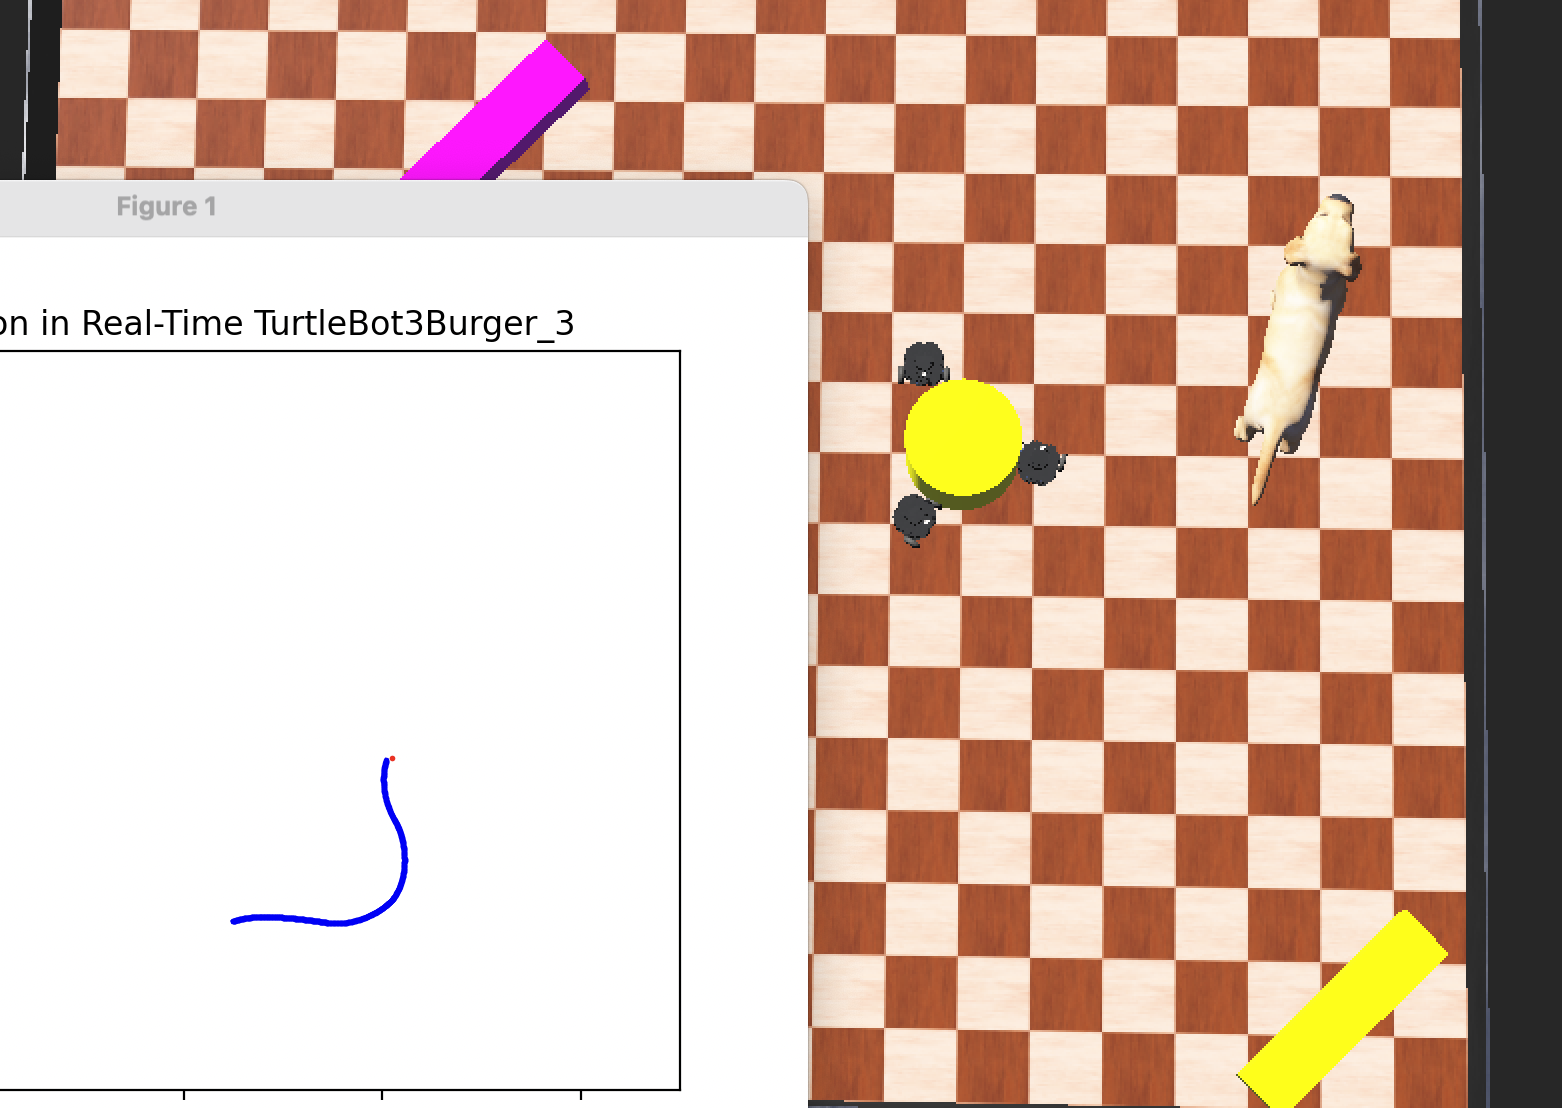
\includegraphics[width=0.5\linewidth]{assets/images/simulation_overview/sim_1.png}
    \caption{Path of the TurtleBotBurger3 after receiving path to follow from the main controller.}
    \label{fig:simulation_overview1} 
\end{figure}

\begin{figure}
    \centering
    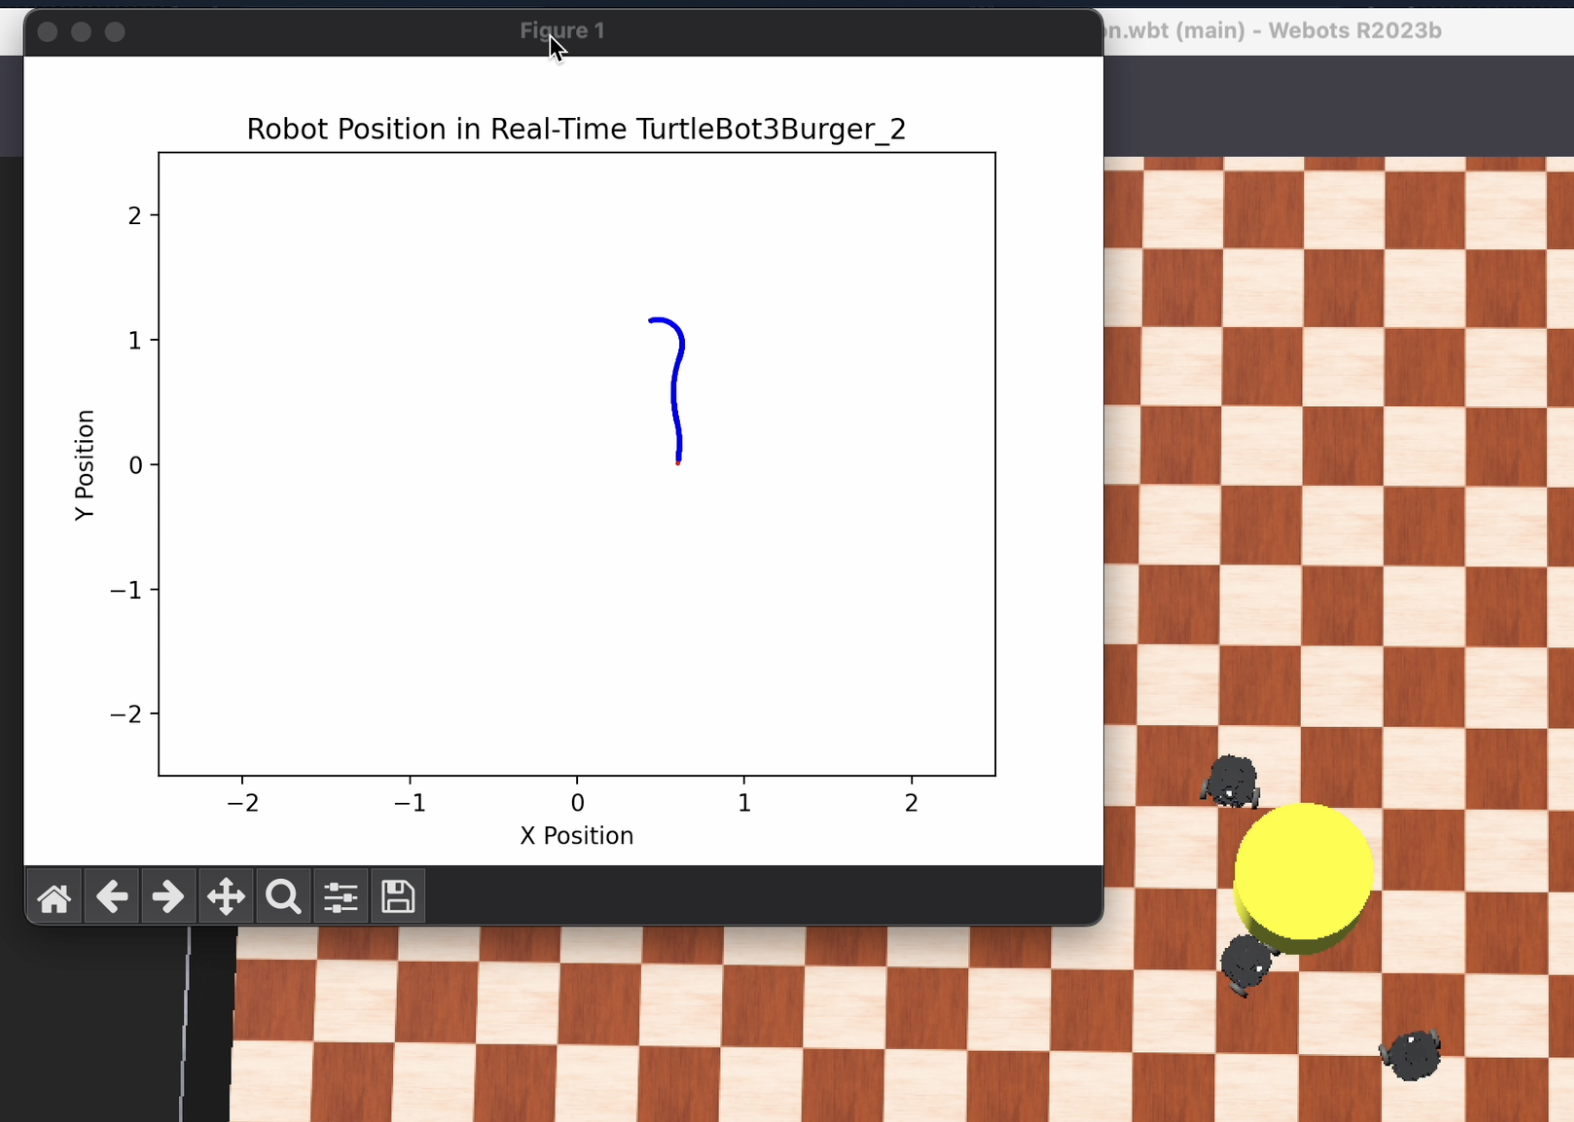
\includegraphics[width=0.5\linewidth]{assets/images/simulation_overview/sim_2.png}
    \caption{3 robots converging to the pre-determined position.}
    \label{fig:simulation_overview2}
\end{figure}

\begin{figure}
    \centering
    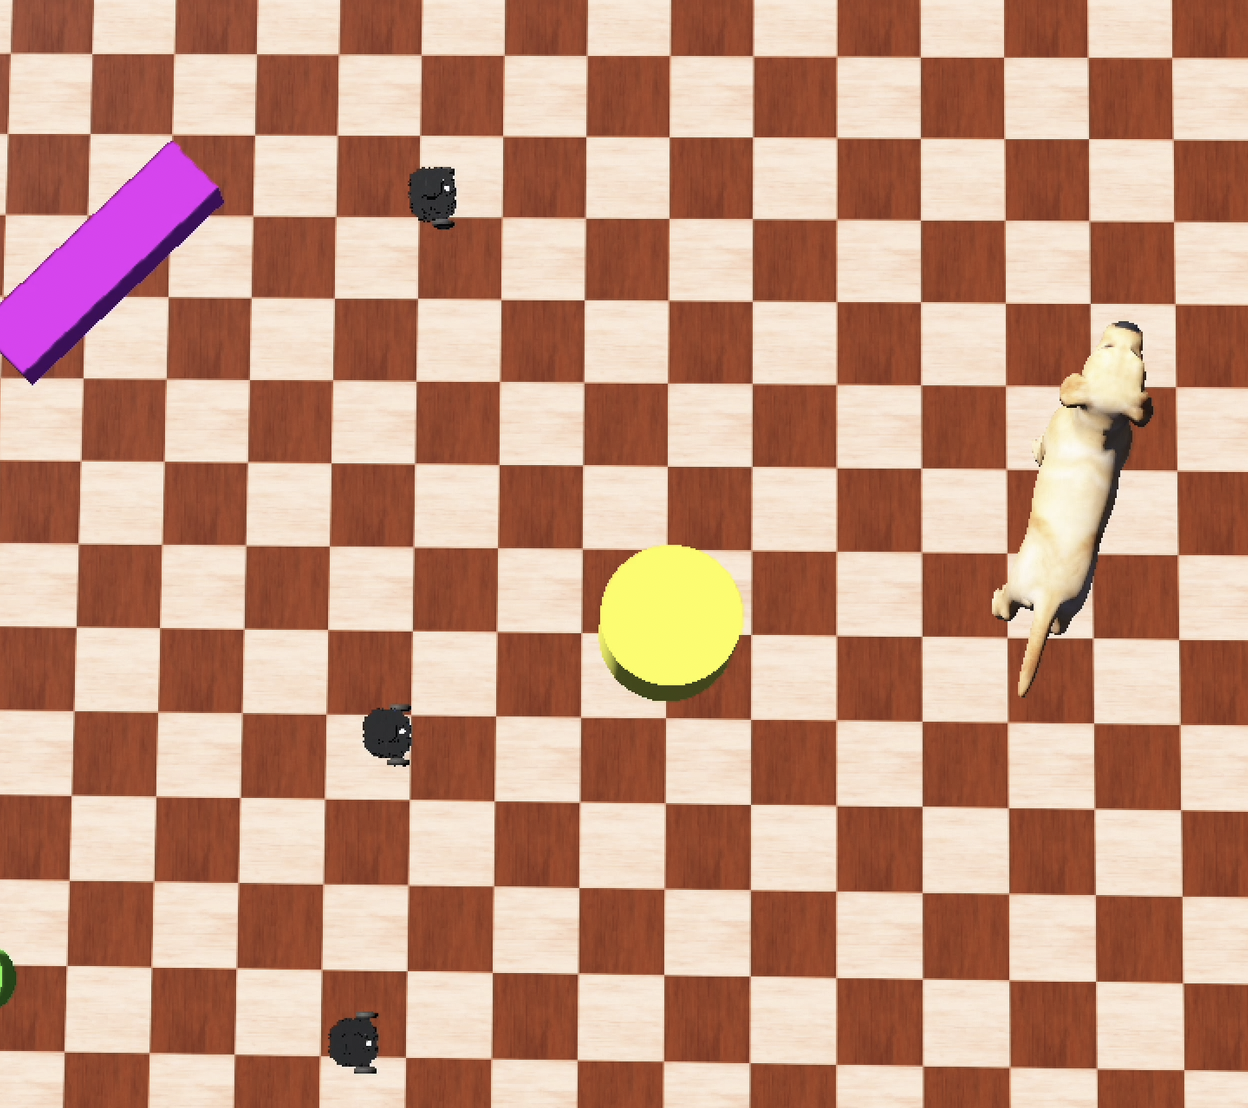
\includegraphics[width=0.5\linewidth]{assets/images/simulation_overview/sim_3.png}
    \caption{3 robots simply moving until an yellow object is found}
    \label{simulation_overview3}
\end{figure}
